\documentclass{article}
\usepackage[utf8]{inputenc}
\usepackage{amsmath}
\usepackage{siunitx}
\usepackage{graphicx}
\usepackage{caption}
\usepackage{subcaption}
\usepackage{float}
\usepackage{enumitem}
\usepackage{amssymb}
\usepackage{pgfplots}
\usepackage[superscript]{cite}
\usepackage{todonotes}
\usepackage{tikz}

\pgfplotsset{compat=1.16}
%\pgfplotsset{
%    dirac/.style={
%        mark=triangle*,
%        mark options={scale=1},
%        ycomb,
%        scatter,
%        visualization depends on={y/abs(y)-1 \as \sign},
%        scatter/@pre marker code/.code={\scope[rotate=90*\sign,yshift=-2pt]}
%    }
%}


\title{Implementation and Review of \\ \textit{``Fast Path-Based Neural Branch Prediction\cite{fastpath}''} \\ NUS CS5222, Project 1}
\author{Luca Krueger}
\date{\today}

\begin{document}
\maketitle
Sniper\cite{carlson2014aeohmcm}

\section{Introduction}

\section{The prediction algorithm}
For simplicity similar variable naming as proposed in the paper is used here:
\begin{align*}
	h: \quad &\text{history length} \\%(keep in mind that all registers related to the history $h$, store $h+1$ values)} \\
	hashlen: \quad &\text{length of the branch adress register} \\
	\hat{x} = \begin{cases} 1 & \text{taken} \\ -1 & \text{not taken} \end{cases} : \quad &\text{speculative prediction outcome} \\
	W \in [0,h] \times [0,hashlen - 1] \times \mathbb{Z}: \quad &\text{weight matrix} \\
	SR \in [0,h]\times \mathbb{Z} : \quad &\text{speculative result history register}  \\
	i = pc \mod hashlen : \quad &\text{hashed branch adress } pc
\end{align*}

For a traditional perceptron predictor a vector of past branching decisions $\hat{x}(t-j) : j \in [0,h-1]$ forms the inputs and is multiplied by a vector of weights $W \in \mathbb{Z}^{h+1}$ and biased by $W[0]$ to calculate the dentritic potential $y(t)$. The perceptrons output is the binary decision $y\geq0 \rightarrow \{\textit{taken}, \textit{not taken}\}$.

The FPBP derives from the traditional perceptron predictor, but introduces some significant structuaral changes. It now uses a two dimensional weight matrix $W$, which might give the first intuition that the single perceptron is now extended to a full single layer of \textit{hashlen} perceptrons, so called Hidden Layer, but this is not the case. Another might intuitively think that the algorithm uses separate perceptrons for different branches within a range of hashed branches, but the outcome of the FPBP does not depend on separate identifiable perceptrons. It depends on a path of previous branches, which is identified by their hashed branch adress. 

This comes with the advantage, that the sum over the path can be calculated iteratively prior to when the final branch decision. The branch outcome for a new branch with hashed branch address $i$ then only depends on the accumulated sum $SR[h]$ biased by $W[i,0]$ and therefore does not cause any additional delay. 
Using the algorithm from the provided code segment of the prediciton function can let us derive the following math.
\begin{align*}
	y = SR[h] + \hat{x} W[i,0] \\
	\textit{prediction} = y\geq 0
\end{align*}
The timing variable $t$ is used to point out the chronological behavior of the algorithm. The function updates $SR[j]$ $\forall j \in [1,h]$ each call.
\begin{align*}
	SR[h-j+1] &= SR[h-j] + \hat{x}(t) W[i(t),j] 
\end{align*}
This can be used to derive a general term for $SR[h]$ in order to trace how the prediction outcome depends on past iterations:
\begin{align*}
	\Rightarrow SR[h] &= SR[h-1] + \hat{x}(t) W[i(t),1] \\
	\iff SR[h] &= SR[h-2] + \hat{x}(t-1) W[i(t-1),2] + \hat{x}(t) W[i(t),1] \\
	\iff SR[h] &= SR[h-3] + \hat{x}(t-2) W[i(t-2),3] + \hat{x}(t-1) W[i(t-1),2] + \hat{x}(t) W[i(t),1] \\
	\iff SR[h] &= SR[h-4] + \hat{x}(t-3) W[i(t-3),4] + \hat{x}(t-2) W[i(t-2),3] + \dots \\% \hat{x}(t-1) W[i(t-1),2] + \hat{x}(t) W[i(t),1] 
	\vdots \quad &= \quad \vdots \\
	\iff SR[h] &= \underbrace{SR[h-h]}_{SR[0] = 0} + \hat{x}(t-h) W[i(t-h),h+1] + \sum_{j=0}^{h-1} \hat{x}(t-j) W[i(t-j),j+1] \\
	\iff SR[h] &=\sum_{j=0}^{h} \hat{x}(t-j) W[i(t-j),j+1] 
\end{align*}
This term shows us, that the cummulative outcome of a sequence does not depend on every single weight (first intuition) nor it depends on a single row of weights corresponging to a single branch address (second intuition). It depends on a sequence of past branch adresses which forms the so called path.

In theory there is a set of ${(hashlen)}^{h}$ detectable distinct paths. In practice, a perfect classification of this set is hard and highly depends on the self adjusting weights. Classification also suffers from aliasing of different paths, because of the hash function. This might result in a changing data set. 

One might also argue, that a sum and a simple threshold classification can also decrease the number of detectable distinct paths, because of the sum's commutative property. Imagine two or more weigths without significant  difference (significant in terms of a difference, which can change to overall outcome) in their values, being permuted without any effect on the branch decision. This reduces the set by all possible permutations regarding these weigths.

The authors proposed to use a threshold $\theta = 1.93 h + 14$, such that $W$ is updated in any case, when the magnitude of y is below this threshold. The value of $\theta$ is empirically determined to give the best result. This results in a higher average magnitude of $W$ \todo{insert snapshot of W} and causes more updates of the weights. Therefore, the chance of pairwise almost equal weights should be reduced. Introducing the threshold indeed slightly improves the prediction accury. 
On the other hand, forcing the magnitude of $W$ to very high values will reduce the flexibility of the learning algoritm as it updates the weights in steps of $+/-1$.
\todo{add mpki for different thresholds}

\section{Comparison}
\todo{output y in update function calculated with res not speculative\_res}
\begin{figure}
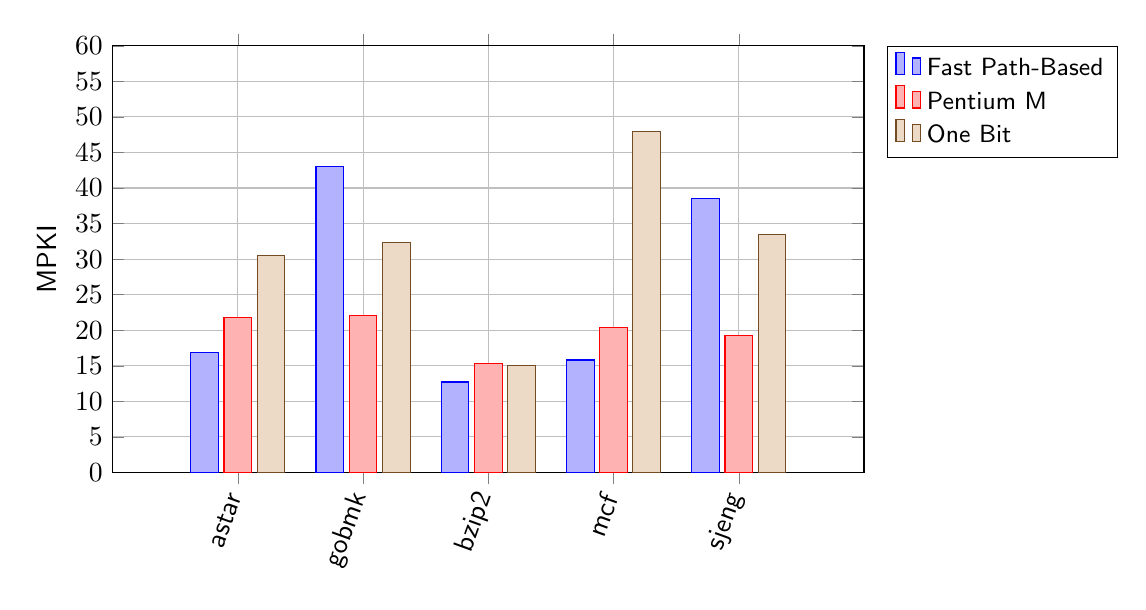
\begin{tikzpicture}
	\begin{axis}[
		width=\textwidth-1cm,
		height=7cm,
		xmin=0, xmax=6,
		ymin=0, ymax=60,
		ylabel=\textsf{MPKI},
		ybar,
		xtick={1,2,3,4,5}, 
		xticklabels={\textsf{astar}, \textsf{gobmk}, \textsf{bzip2}, \textsf{mcf}, \textsf{sjeng}},
		ytick distance ={5},
		xmajorgrids=true,
		ymajorgrids=true,
		x tick label style={rotate=70,anchor=east},
		legend pos=outer north east,
		legend cell align=left,
		legend style={font=\small\sf}
	]
		% own BP
		\addplot
			coordinates {(1,16.84) (2,42.98) (3,12.72) (4,15.81) (5,38.56)};

		% pentium_m
		\addplot
			coordinates {(1,21.79) (2,22.12) (3,15.26) (4,20.43) (5,19.27)};

		% one_bit size 1024
		\addplot
			coordinates {(1,30.45) (2,32.30) (3,15.04) (4,48.00) (5,33.50)};

		\legend{Fast Path-Based, Pentium M, One Bit}
	\end{axis}
\end{tikzpicture}
\caption{MKPI Plot: FPBP compared to Sniper's\cite{carlson2014aeohmcm} build-in branch predictors}
\end{figure}


\section{Verification}
The implementation of the FPBP does not perform as well as promised in the paper. The accuracy is significantly lower than the authors implementation showed in their benchmarks. This might lead to think that the implementation is simply wrong or consists of some tiny mistakes. 
In earlier stages, before debugging, my implementation indeed consisted of a few mistakes. For example, first the branch prediction history and weights were misaligned by one position. Errors like these result in a branch prediction accuracy not significantly better than a random guess. This, and the fact that the neural predictor indeed performs with very high accuracy for some parts during a running application, whereas it does not for other parts, should reduce the chance that the accuracy still suffers from bad mistakes to a negligible amount.
\bibliography{references}
\bibliographystyle{unsrt}
\end{document}
